%%% Choose between 16:9 and 4:3 format by commenting out/uncommenting one of the following lines:
\documentclass[aspectratio=169]{beamer} % 16:9
% \documentclass{beamer} % 4:3

%=========================================================================================================================

\usepackage[english]{babel}     % English language
\usepackage[latin1]{inputenc}   % Input encoding
\usepackage{tikz}               % For creating graphics
\usepackage[mode=buildnew]{standalone}
\usepackage{url}                % For including urls
\usepackage{tabularx}           % For better tables
\usepackage{xcolor}             % Für bunte Farbe :)

\usetheme{aig}                  % Set beamer theme

%=========================================================================================================================
\title{Qualit\"at von Wikipedia-Artikeln}

% \author[S. Author]{Some Author}
\institute{Artificial Intelligence Group,\\
University of Hagen, Germany}
\date{\today}
%=========================================================================================================================
\logo{
\includegraphics[width=3cm]{figures/logoaig.png}}
%=========================================================================================================================

\begin{document}

%=========================================================================================================================

% frame
% block
% alertblock
% exampleblock

% \highlight{}
% \darkhighlight{}
% \yellowhighlight{}
% \mathhighlight{}
% \darkmathhighlight{}
% \yellowmathhighlight{}

% appendix

\begin{frame}
    \titlepage
\end{frame}
\nologo

\section{Problemstellung}

\begin{frame}{Problemstellung}
    \textcolor{red}{Beispiel Wikipedia-Artikel mit promo}
\end{frame}

\begin{frame}{Problemstellung}
    \begin{block}{Problemstellung}
        Das Ziel dieses Projekts ist die Entwicklung von Modellen zur automatisierten Klassifikation von Wikipedia-Artikeln als promotional (werblich) oder nicht-promotional. Wikipedia strebt nach objektiven und neutralen Inhalten; daher ist die Identifizierung von Artikeln mit werbenden Charakter von gro\ss{}er Bedeutung, um die sachliche Qualit\"at der Plattform zu gew\"ahrleisten.
    \end{block}
    \textcolor{red}{TODO: Konkret als Frage formulieren?\\ Zweite Frage ergänzen: Warum ist der Artikel nicht neutral?}
\end{frame}

\section{Daten}

\begin{frame}{Daten}
    \begin{itemize}
        \item 54116 gelabelte Wikipedia Artikel

        \item 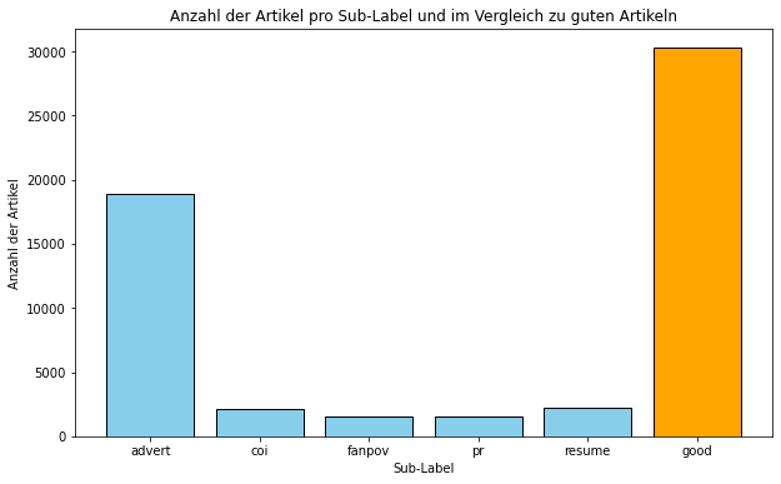
\includegraphics[width=10cm]{figures/distribution_multiple_classes.png}
    \end{itemize}
\end{frame}


\begin{frame}{Weitere Daten}
    \textcolor{red}{TODO: Ans Ende verschieben; Ausblick?}
    \begin{block}{Weitere Daten}
        \begin{itemize}
            \item Wikipedia-Dump
            \item Versuche Daten zu Augmentieren
            \item Suche nach Fanpages, Wissenschaftlichen Artikeln usw.
        \end{itemize}
    \end{block}
\end{frame}


\section{Ans\"atze}

\subsection{Logistische Regression}

\begin{frame}{Logistische Regression (1)}
    \begin{block}{Datenvorverarbeitung}
        \begin{itemize}
            \item Entfernung von Sonderzeichen und Kleinbuchstabierung (nativ durch TF-IDF-Vektorisierung)
            \item Stopw\"orter entfernt, aber Zahlen beibehalten
            \item Optimierung der TF-IDF-Vektorisierung durch Gridsearch:
                  \begin{itemize}
                      \item Maximale Anzahl von Features: \{5000, \textbf{10000}, 20000\}
                      \item n-Gramm-Bereich: \{(1,1), (\textbf{1,2}), \dots ,(3,4)\}
                  \end{itemize}
        \end{itemize}
    \end{block}
\end{frame}

\begin{frame}{Logistische Regression (2)}
    \begin{block}{Methode}
        \begin{itemize}
            \item Klassifikation mit \texttt{LogisticRegression}:
                  \begin{itemize}
                      \item Solver: \texttt{lbfgs}, \texttt{saga}
                      \item Strafterm: \(L1\) oder \(L2\)-Regularisierung
                      \item Multi-Class: \texttt{OneVsRestClassifier} f\"ur multilabel-Klassifikation
                  \end{itemize}
            \item Optimierung des Modells:
                  \begin{itemize}
                      \item Gridsearch f\"ur Hyperparameter der logistischen Regression:
                            \begin{itemize}
                                \item Regularisierungsparameter \(C\): \{0.01, 0.1, 1, 10, 100\}
                                \item Verschiedene Solver (\texttt{lbfgs}, \texttt{saga})
                            \end{itemize}
                      \item Umgang mit Klassenungleichgewicht: Easy Data Augmentation (EDA) mit nltk.
                            \begin{itemize}
                                \item Synonym Replacement: Es werden zuf\"allig n W\"orter durch Synonyme ersetzt und als neuer Text mit gleichem Label ausgegeben.
                                \item In Pr\"ufung: Random Swap, Random Insertion und Random Deletion
                            \end{itemize}
                  \end{itemize}
        \end{itemize}
    \end{block}
\end{frame}

\begin{frame}{Fortschritte durch bisherige Augmentierung}
    \definecolor{mattegreen}{RGB}{120,180,120} % Mattes Grün
    \definecolor{grey}{RGB}{150,150,150} % Dezentes Grau
    \begin{block}{Verbesserung der Erkennungsraten (Recall) durch Augmentierung}
        \begin{columns}[T,onlytextwidth]
            \column{0.48\textwidth}
            \textbf{Sublabel: advert}
            \begin{itemize}
                \item Original: 0.949
                \item Augmented: 0.900 \tikz[baseline]{\node[anchor=base] {\textcolor{red}{$\searrow$}};}
            \end{itemize}
            
            \textbf{Sublabel: coi}
            \begin{itemize}
                \item Original: 0.000
                \item Augmented: 0.016 \tikz[baseline]{\node[anchor=base] {\textcolor{grey}{$\nearrow$}};}
            \end{itemize}
            
            \textbf{Sublabel: resume}
            \begin{itemize}
                \item Original: 0.408
                \item Augmented: 0.526 \tikz[baseline]{\node[anchor=base] {\textcolor{grey}{$\nearrow$}};}
            \end{itemize}
            
            \column{0.48\textwidth}
            \textbf{Sublabel: fanpov}
            \begin{itemize}
                \item Original: 0.195
                \item Augmented: 0.427 \tikz[baseline]{\node[anchor=base] {\textcolor{mattegreen}{$\uparrow$}};}
            \end{itemize}
            
            \textbf{Sublabel: pr}
            \begin{itemize}
                \item Original: 0.000
                \item Augmented: 0.008 \tikz[baseline]{\node[anchor=base] {\textcolor{grey}{$\nearrow$}};}
            \end{itemize}
        \end{columns}
    \end{block}
\end{frame}

\subsection{Support Vector Machine}

\begin{frame}{Support Vector Machine (1)}
    \begin{block}{Datenvorverarbeitung}
        \begin{itemize}
            \item Zusammenf\"uhren der CSV-Dateien
            \item Entfernen \"uberfl\"ussiger Features
        \end{itemize}
    \end{block}
\end{frame}

\begin{frame}{Support Vector Machine (2)}
    \begin{block}{Methode}
        \begin{itemize}
            \item TF-IDF-Vektorisierung
            \item Vergleich verschiedener Kernels:
                \begin{itemize}
                    \item \texttt{linear}, \texttt{poly}, \texttt{rbf}, \texttt{sigmoid}.
                    \item Keine Vorteile gegen\"uber \texttt{linear} festzustellen.
                    \item \texttt{LinearSVC} mit deutlich geringerer Laufzeit.
                    \item Parameter-Tuning mit \texttt{GridSearchCV}.
                \end{itemize}
            \item \textbf{Bin\"are Klassifikation}:
                \begin{itemize}
                    \item \texttt{LinearSVC} liefert Precision, Recall, F1-Score und Accuracy jeweils 0.96 - 0.97.
                \end{itemize}
            \item \textbf{Multilabel-Klassifikation}:
                \begin{itemize}
                    \item Klassifikation mit \texttt{MultiOutputClassifier} und \texttt{LinearSVC}.
                    \item Nur \texttt{advert} einigerma\ss{}en identifizierbar mit F1-Score 0.86.
                    \item Bei \texttt{coi}, \texttt{fanpov}, \texttt{pr}, \texttt{resume} F1-Scores von 0.00 bis 0.45.
                    \item Nicht-lineare Kernels liefern \"ahnliche Ergebnisse.
                \end{itemize}
        \end{itemize}
    \end{block}
\end{frame}

\subsection{Bayes Klassifikator}

\begin{frame}{Bayes Klassifikator (1)}
    \begin{block}{Datenvorverarbeitung}
        \begin{itemize}
            \item Entfernen von Nicht-Wort-Zeichen
            \item Umwandlung in Kleinbuchstaben
            \item Entfernung von f\"uhrenden und folgenden Leerzeichen
            \item Beibehaltung von Stoppw\"ortern und Zahlen (KPIs nicht beeinflusst)
        \end{itemize}
    \end{block}
\end{frame}
\begin{frame}{Bayes Klassifikator (2)}
    \begin{block}{Methode}
        \begin{itemize}
            \item Textrepr\"asentation mittels TF-IDF-Vektorisierung:
                  \begin{itemize}
                      \item Maximale Anzahl von Features: 10.000
                      \item n-Gramm-Bereich: Unigramme (1,1)
                      \item Minimale Dokumentenfrequenz (\texttt{min\_df}): 0.001
                      \item Maximale Dokumentenfrequenz (\texttt{max\_df}): 0.9
                  \end{itemize}
            \item Einstellung des Gl\"attungsparameters \(\alpha = 1.0\)
            \item \textbf{Bin\"are Klassifikation}:
                  \begin{itemize}
                      \item Einsatz von \texttt{MultinomialNB} f\"ur die Klassifikation zwischen promotional und nicht-promotional Artikeln
                  \end{itemize}
            \item \textbf{Multilabel-Klassifikation}:
                  \begin{itemize}
                      \item Verwendung von \texttt{OneVsRestClassifier} mit \texttt{MultinomialNB} f\"ur die Klassifikation in mehrere Klassen
                      \item Behandlung des Klassenungleichgewichts durch Oversampling mit \texttt{RandomOverSampler}
                  \end{itemize}
        \end{itemize}
    \end{block}
\end{frame}
\begin{frame}{Bayes Klassifikator (3)}
    \begin{block}{Ergebnisse}
        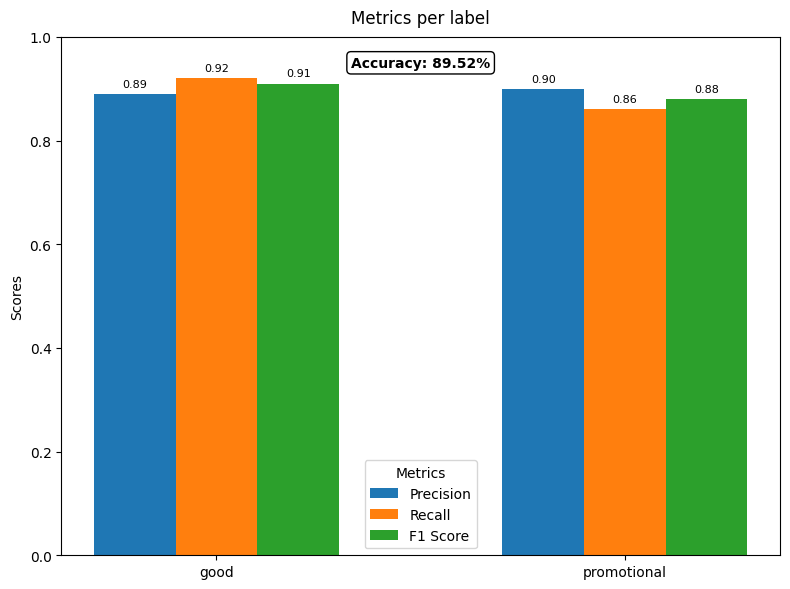
\includegraphics[width=6.8cm]{figures/evaluation_nbb.png} 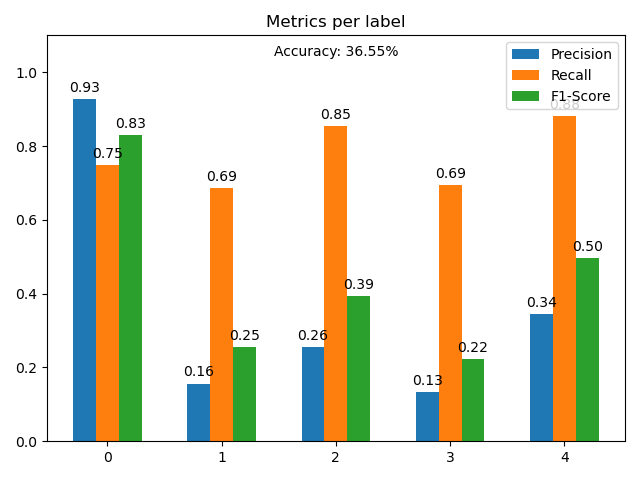
\includegraphics[width=6.8cm]{figures/evaluation_nbm.png}
    \end{block}
\end{frame}

\subsection{Convolutional Neural Network}

\begin{frame}{Convolutional Neural Network}
    \begin{block}{Idee}
    \begin{itemize}
        \item Position von relevanten Textbausteinen im Text ist nicht wichtig

        \item nutze Filter um relevante Textbausteine zu finden
        \begin{figure}
            \centering
            \includestandalone[width=12cm]{figures/conv1d}
        \end{figure}
    \end{itemize}
    \end{block}
\end{frame}

\begin{frame}{Convolutional Neural Network}
    \begin{block}{Datenvorverarbeitung}
        \begin{itemize}
            \item Tokenisierung mittels Byte Pair Encoding (cl100kbase)

            \includestandalone[width=12cm]{figures/tokenization}

            \textcolor{red}{Tokens to number}
    
            \item Konvertierung in Tensor f\"ur pytorch Datensatz 
        \end{itemize}
    \end{block}
\end{frame}

\begin{frame}{Convolutional Neural Network}
    \begin{block}{Faltung}
        \begin{itemize}
            \item Embedding Layer
        
            \item \textcolor{red}{Bild von 1d Faltung auf Embedding Layer}

            \item Pooling Layer
        \end{itemize}
    \end{block}
\end{frame}

\begin{frame}{Convolutional Neural Network}
    \begin{block}{Training/Optimierung}
        \begin{itemize}
            \item Viele Hyperparameter
            \begin{itemize}
                \item Tokenizer

                \item Embedding Dimension

                \item Anzahl Conv Layers

                \item FFN
            \end{itemize}
            
            \item GridSearch
        \end{itemize}
    \end{block}
\end{frame}

\subsection{5.Ansatz}
\begin{frame}
    \begin{block}{Ideen 5. Ansatz}
        \begin{itemize}
            \item Graph der Beziehungen der Daten untereinander Darstellt
            \item Imitierung der Embeddings durch Gram-Schmidt-Verfahren
                  \begin{itemize}
                      \item Erste Versuche bereits gemacht
                  \end{itemize}
            \item Vortrainierte Embeddings, als Eingabe f\"ur andere Methoden des maschiniellen Lernens verwenden.
        \end{itemize}
    \end{block}
\end{frame}

\section{Zusammenfassung}
\begin{frame}
    \begin{block}{Zusammenfassung}
        \begin{itemize}
            \item Gemachte Arbeit
                  \begin{itemize}
                      \item 3 Klassische Verfahren implementiert
                      \item CNN implementiert
                      \item Erste Auswertungen gemacht
                      \item F\"unfter Ansatz: erste Ideen gesammelt und Experimente gemacht
                  \end{itemize}
            \item Probleme
                  \begin{itemize}
                      \item Ungleiche Verteilung der Daten
                  \end{itemize}
            \item N\"achste Schritte
                  \begin{itemize}
                      \item Parameter der Klassischen Verfahren Anpassen
                      \item Parameter des CNN anpassen
                      \item Weitere Ideen f\"ur f\"unften Ansatz finden/erg\"anzen
                            ausdenken bzw. weiter testen
                      \item Weitere Datens\"atze finden bzw. Vorbereiten
                  \end{itemize}
        \end{itemize}
    \end{block}
\end{frame}

\end{document}
